\chapter{State of the art}
In this chapter, we will explore the state of the art. In the first section, we  will first discuss the important variations of double pendulum that is widely used by the research society. Subsequently, we will delve into the basic dynamics of a double pendulum system. In the second section, we will review some of the most renowned works related to learning-based control in the field of robotics.

\section{Theory}
In this section, we will explore the fundamental principles governing the dynamics of a double pendulum.

Broadly speaking, a double pendulum system is a mechanical structure consisting of two pendulum arms or masses suspended independently, allowing them to swing freely. These pendulum arms are typically connected in series, with the motion of the second pendulum influenced by the motion of the first.

Double pendulum setups take various forms, including the widely researched double inverted pendulum on a cart (DIPC) [1] and the Furuta pendulum [2][3]. The double pendulum used in this thesis is relatively simple, comprising two links connected in series by revolute joints. Unlike the Furuta pendulum, both links of the double pendulum move in the same plane within three-dimensional space. These links are also connected to the world frame via revolute joints. In contrast to the DIPC setup, the actuation capability is solely limited by the torque that the joints can generate, unrestricted by the length of a prismatic rail. We will discuss the dynamics of the double pendulum system in the following section.

As shown in Figure \ref{fig:double pendulum dynamics}, we model the dynamics of the double pendulum with 15 parameters which include 8 link parameters namely masses \((m_1,m_2)\)
, lengths \((l_1,l_2)\)
, center of masses \((r_1,r_2)\) 
, inertias \((I_1,I_2)\)
 for the two links, and 6 actuator parameters namely motor inertia \(I_r\)
, gear ratio \(g_r\)
, coulomb friction \((c_{f1},c_{f2})\)
, viscous friction \((b_1,b_2)\)
 for the two joints and gravity \(g\).
\begin{figure}[h]
  \centering
  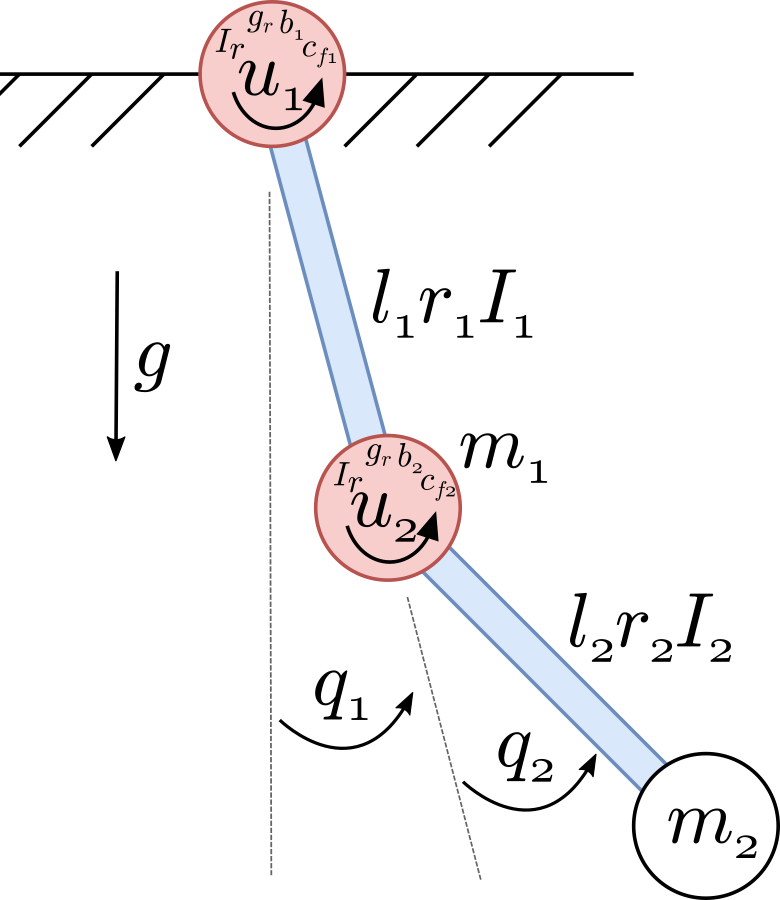
\includegraphics[width=0.5\textwidth]{figures/double_pendulum_dynamics.png} % Replace "example-image" with the actual image file name and path
  \caption{Double pendulum dynamics\cite{double_pendulum_dynamics}}
  \label{fig:double pendulum dynamics}
\end{figure}

The generalized coordinates \( \mathbf{q} =[q_1,q_2]^T \) are the joint angles measured from the free hanging position. The state vector of the systems contains the position coordinates and their time derivatives: \(\mathbf{x}=[\mathbf{q},\mathbf{\dot{q}}]^T\). The torque applied by the actuators are \(\mathbf{u}=[u_1,u_2]\). The equation of motion for the dynamics of a dynamical system can be derived following the blow steps:

\textbf{Step 1. Define the Lagrangian (\(L\)):}

   The Lagrangian (\(L\)) is defined as the difference between the kinetic energy (\(T\)) and the potential energy (\(U\)) of the system:
   \begin{align}
         L = T - U
   \end{align}


\textbf{Step 2. Express the Kinetic Energy (\(T\)):}

   The kinetic energy (\(T\)) of the double pendulum is the sum of the kinetic energies of both links. The kinetic energy for a link is given by:
   \begin{align}
        \label{eq:kinetic energy}
        T = \frac{1}{2} m_1 (\dot{x}_1^2 + \dot{y}_1^2) + \frac{1}{2} m_2 (\dot{x}_2^2 + \dot{y}_2^2)
   \end{align}

   where \(m_1\) and \(m_2\) are the masses of the links, \((x_1, y_1)\) and \((x_2, y_2)\) are their positions, and \(\dot{x}_1, \dot{y}_1, \dot{x}_2, \dot{y}_2\) are their respective velocities.

\textbf{Step 3. Express the Potential Energy (\(U\)):}

   The potential energy (\(U\)) of the double pendulum is the sum of the potential energies of both links. The potential energy for a link in a gravitational field is given by:
   \begin{align}
         \label{eq:potential energy}
         U = m_1 g y_1 + m_2 g y_2
   \end{align}

   where \(g\) is the acceleration due to gravity.
   
   
\textbf{Step 4. Formulate the Lagrange's Equation:}

  The equations of motion (EoM) for joint coordination \(q\) are derived using Lagrange's equation:

    \begin{align}
    \label{eq:lagrange equation}
    \frac{d}{dt} \left(\frac{\partial L}{\partial \dot{q_i}}\right) - \frac{\partial L}{\partial q_i} = 0
    \end{align}

\textbf{Step 5. Solve the Equations of Motion:}

    The set of second-order differential equations obtained is solved to determine the system's equations of motion. The system dynamics, including friction, are represented as follows:
   
   \begin{align}
        \label{eq:EoM}
        M(q)\ddot{q} + C(q,\dot{q})\dot{q} &= Du + G(q) - F(\dot{q})
   \end{align}
    
    Expressing the equation of motion in terms of the state vector \(\mathbf{x}=[\mathbf{q},\mathbf{\dot{q}}]^T\), we have:
    
    \begin{equation}
    \begin{split}
        \dot{x} &= f(x,u) \\
        &= \begin{bmatrix} 
            \dot{q} \\ 
            M^{-1}(Du - C(q,\dot{q})\dot{q} + G(q) - F(\dot{q})) 
       \end{bmatrix}
    \end{split}
    \end{equation}

   Considering the forward kinematics of the double pendulum system, the Cartesian coordinates of the joint between the first and second links are represented as \(P_1=(x_1,y_1)\), while the coordinates of the end effector are represented as \(P_2=(x_2,y_2)\). These Cartesian coordinates can be expressed in terms of the joint coordinates \(q\) as follows:

    \begin{align}
        \label{eq:p1}
        \left\{
        \begin{aligned}
        x_1 &= l_1 \sin(q_1) \\
        y_1 &= - l_1 \cos(q_1)
        \end{aligned}
        \right.
    \end{align}

    \begin{align}
        \label{eq:p2}
        \left\{
        \begin{aligned}
        x_2 &= l_1 \sin(q_1) + l_2 \sin(q_1 + q_2) \\
        y_2 &= -l_1 \cos(q_1) - l_2 \cos(q_1 + q_2)
        \end{aligned}
        \right.
    \end{align}

    Substituting Equation \ref{eq:p1} and \ref{eq:p2} into \ref{eq:kinetic energy}, \ref{eq:potential energy}, \ref{eq:lagrange equation}, and \ref{eq:EoM}, we can derive the mass matrix (where \(s_1 = \sin(q_1), c_1 = \cos(q_1), \ldots\)).
    \begin{equation}
    \mathbf{M} =
    \left[ 
    {\begin{array}{cc}
    I_1 + I_2 + l_1^2m_2 + 2l_1m_2r_2c_2 + g_r^2I_r + I_r  &   I_2 + l_1m_2r_2c_2 - g_rI_r  \\
    I_2 + l_1m_2r_2c_2 - g_rI_r                    & I_2 + g_r^2I_r                       \\
    \end{array}} 
    \right]
    \end{equation}
    
    The Coriolis matrix:
    
    \begin{equation}
    \begin{split}
    \mathbf{C} = \left[
    \begin{matrix}
    -2 \dot{q}_2 l_{1} m_{2} r_{2} \sin(q_2) & -\dot{q}_2 l_{1} m_{2} r_{2} \sin(q_2)\\
    \dot{q}_1 l_{1} m_{2} r_{2} \sin(q_2) & 0
    \end{matrix}
    \right],
    \label{eq:coriolis_matrix}
    \end{split}
    \end{equation}
    
    The gravity vector:
    
    \begin{equation}
    \begin{split}
    \mathbf{G} = \left[
    \begin{matrix}
    - g m_{1} r_{1} \sin(q_1) - g m_{2} \left(l_{1} \sin(q_1) + r_{2} \sin(q_{1+2}) \right) \\
    - g m_{2} r_{2} \sin(q_{1+2})
    \end{matrix}
    \right],
    \label{eq:gravity_matrix}
    \end{split}
    \end{equation}
    
    The friction vector:
    
    \begin{equation}
        \begin{split}
            \mathbf{F} =
            \left[
                \begin{matrix}
                    b_1 \dot{q}_1 + c_{f1} \arctan(100\,\dot{q}_1) \\
                    b_2 \dot{q}_2 + c_{f2} \arctan(100\,\dot{q}_2)
                \end{matrix}
            \right]
        \end{split}
        \label{eq:friction_function}
    \end{equation}
    (the \(\arctan(100\,\dot{q}_i)\) function is used to approximate the discrete step function for the coulomb friction)

    And the actuator selection matrix \(\mathbf{D}\):
    
    \begin{equation}
        \begin{split}
            \mathbf{D}_{full} =
            \left[
                \begin{matrix}
                    1 & 0 \\
                    0 & 1
                \end{matrix}
            \right],
            \quad
            \mathbf{D}_{pendu} =
            \left[
                \begin{matrix}
                    1 & 0 \\
                    0 & 0
                \end{matrix}
            \right],
            \quad
            \mathbf{D}_{acro} =
            \left[
                \begin{matrix}
                    0 & 0 \\
                    0 & 1
                \end{matrix}
            \right]
        \end{split}
    \end{equation}
    
    for the fully actuated system, the pendubot or the acrobot.

\section{Related work}
This thesis focuses on learning-based robotic motion control, a field that has garnered increasing attention in recent years, with significant contributions from various research institutes.

Today, much of the research in this field is conducted within simulation environments due to their cost-effectiveness and the ability to facilitate rapid iteration. One noteworthy project from 2018 is the DeepMimic project\cite{peng2018deepmimic}, undertaken by researchers at the University of California, Berkeley. This work resides at the intersection of deep reinforcement learning, imitation learning, and robotics.

The DeepMimic project utilizes physics-based simulations to successfully replicate the diverse range of behaviors exhibited in the real world by 3D characters. These characters include real-world examples such as humanoid and Atlas robotics, as well as fictional characters like T-Rexes and dragons. Instead of relying on manually designed controllers, the project employs deep reinforcement learning methods to generalize to new skills and situations, often without human intervention.

In the training process, the agent is provided with reference data recorded by motion capture actors or keyframed animations. Through imitation learning, the agent is guided to achieve specific predefined goals. The central contribution of this project lies in its framework, which combines goal-directed reinforcement learning with reference data generated by humans. This combination enables the imitation of a wide variety of motion skills.

\begin{figure}[H]
  \centering
  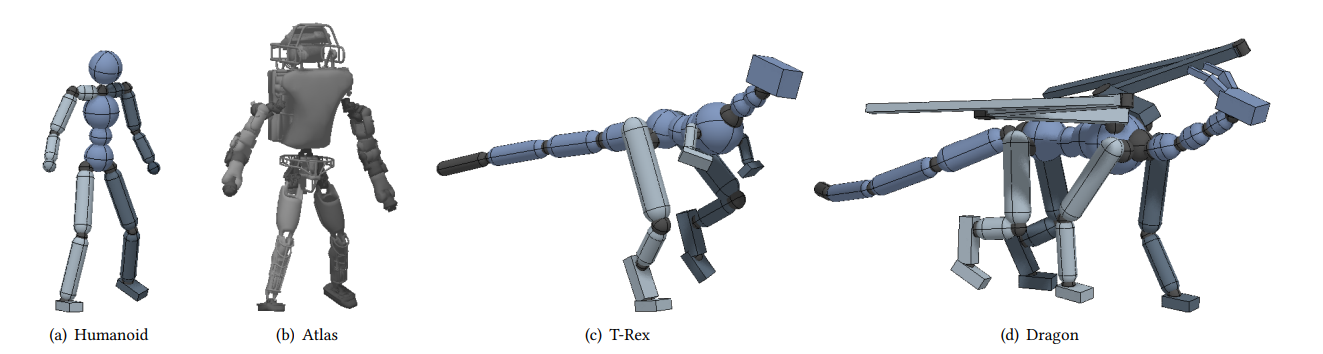
\includegraphics[width=1.1\textwidth]{figures/deepmimic.png} % Replace "example-image" with the actual image file name and path
  \caption{3D characters in Deepmimic project\cite{peng2018deepmimic}}
  \label{fig:deepmimic}
\end{figure}

In the context of reinforcement learning, a distinction exists between model-free and model-based approaches. Model-free reinforcement learning(MFRL) does not require information about the transition model, whereas model-based reinforcement learning(MBRL) leverages the transition model to make decisions based on a prior known model or one learned from interactions.

The model-free approach is notably characterized by its sample inefficiency. Successful training often takes many hours, if not days or weeks.

An intriguing project that relies solely on model-free deep reinforcement learning is the Learning-to-Walk-in-20 Minutes project\cite{smith2022walk} conducted by researchers from UC Berkeley. They employ an algorithmic framework closely related to DroQ \cite{hiraoka2021dropout}, an extension of the SAC algorithm \cite{haarnoja2018soft} incorporating dropout \cite{srivastava2014dropout} and layer normalization \cite{ba2016layer}. Remarkably, their training is conducted directly on the real system. They demonstrate that current deep RL methods can effectively teach quadrupedal locomotion in under 20 minutes, a stark contrast to previous research conducted by Kumar et al. \cite{kumar2021rma}, which employed the same hardware but required \(1.2 \times 10^9\) samples to train a robust controller for locomotion. This corresponds to roughly 4.5 months' worth of cumulative experience.

Model-based reinforcement learning is recognized for its integration of an environment model with trial-and-error learning. One notable advantage is the potential for higher sample efficiency compared to the model-free approach. This work, conducted by the University of Toronto\cite{wang2019benchmarking}, provides a comprehensive comparison by benchmarking model-based reinforcement learning.

\begin{figure}[H]
  \centering
  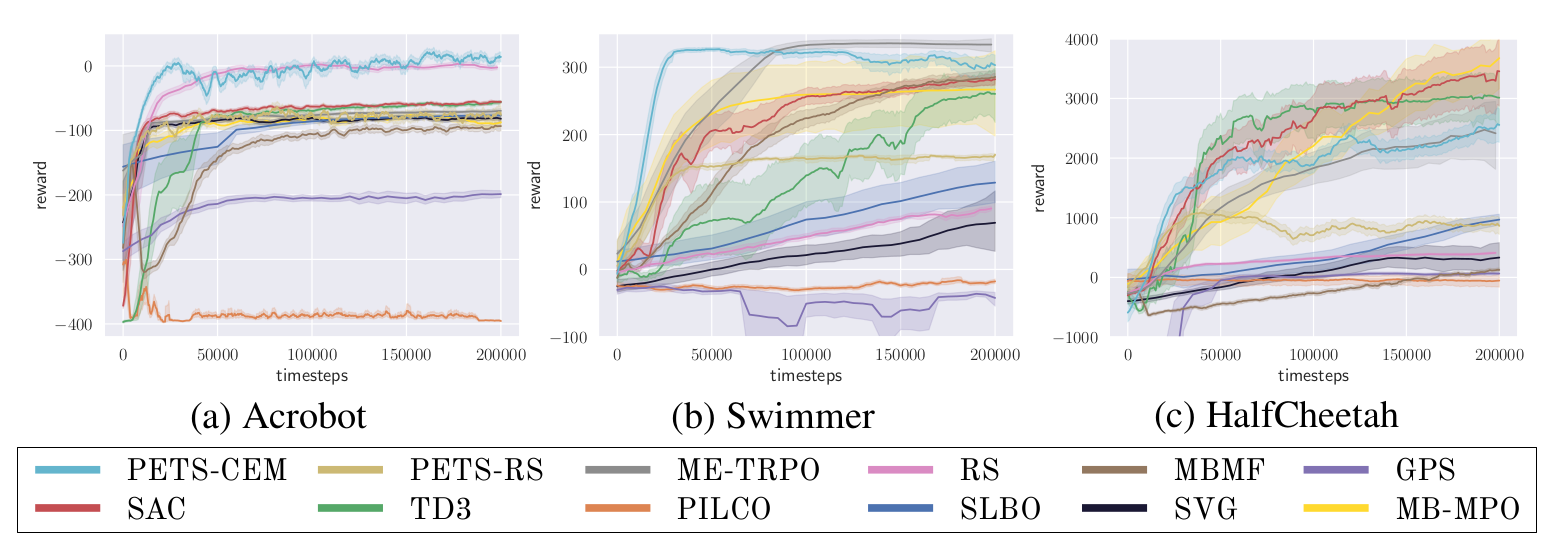
\includegraphics[width=0.9\textwidth]{figures/benchmarking_mbrl.png} % Replace "example-image" with the actual image file name and path
  \caption{Benchmarking model-based reinforcement learning\cite{wang2019benchmarking}}
  \label{fig:benchmarking MBRL}
\end{figure}

The team has collected 11 Model-Based Reinforcement Learning (MBRL) algorithms and 4 Model-Free Reinforcement Learning (MFRL) algorithms across 18 benchmarking environments specifically designed for MBRL in simulation. These benchmarking environments are based on the standard OpenAI Gym\cite{brockman2016openai}, ranging from simple 2D tasks like cart-pole to complex setups like humanoid. The benchmarking process is further extended by introducing noise into the environment, including disturbances in observations and actions.

The team has discovered that while 1 million time-step training is common for MFRL algorithms, many MBRL algorithms converge much earlier, often within 200k time-steps. Within the field of MBRL, when it comes to the evaluation of sample efficiency, asymptotic performance, and robustness, there is no clear and consistent best MBRL algorithm. This leaves ample opportunities for future research to leverage the strengths of different approaches.

Another notable challenge in reinforcement learning-based robotic control is the sim-to-real gap problem. Since agents are typically trained in carefully designed simulated worlds, these simulations can sometimes be idealized or oversimplified to some extent. Consequently, the optimal policy derived from the simulation often fails to account for the uncertainties of the real world, leading to failures when executing intended tasks. There are several approaches to bridging the sim-to-real gap, and the following work presents an interesting approach.

A research team from ETH Zurich has made significant progress in addressing the sim-to-real interface challenge \cite{hwangbo2019learning}. Their methodology involves training a control model for a quadruped robot within a simulation environment. By utilizing a neural network and leveraging data collected from the real robot, they approximated the dynamics model of the physical robot. This approach has facilitated the accurate implementation of the control policy derived from the virtual environment onto the real robot. These exemplary works demonstrate the promising applications of learning-based approaches in various aspects of robot control.

\begin{figure}[H]
  \centering
  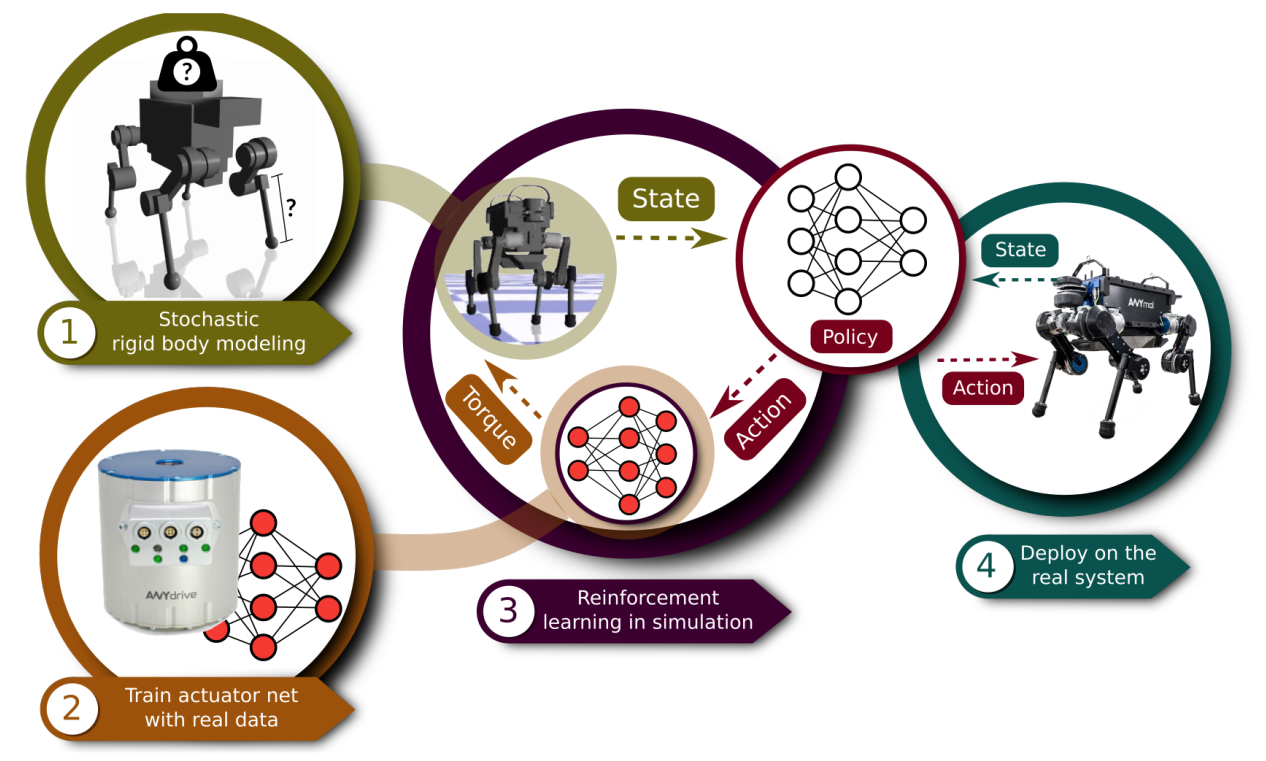
\includegraphics[width=0.9\textwidth]{figures/quadruped_sim2real.png} % Replace "example-image" with the actual image file name and path
  \caption{Sim-to-real framework for RL-based quadruped controller\cite{hwangbo2019learning}}
  \label{fig:benchmarking MBRL}
\end{figure}

In conclusion, in the field of reinforcement learning-based control in robotics, researchers currently face three major challenges:

\begin{enumerate}
    \item \textbf{Sample Inefficiency in Model-Free Reinforcement Learning:}
    
    Model-free reinforcement learning is known for its sample inefficiency, where the time required for random trial and error can be excessively long.
    
    \item \textbf{Immaturity of Model-based RL} 
    
    Model-based reinforcement learning is a growing force but still in its infancy. Finding the right balance between model information and reinforcement learning remains an ongoing challenge.
    
    \item \textbf{Sim-to-Real Gap Limitations:} 
    
    Deploying controllers learned through reinforcement learning on real systems is limited due to the significant sim-to-real gap. This limitation confines a substantial portion of research to simulations.
\end{enumerate}

The research community has much work to do before reinforcement learning becomes a stable and widely accepted approach in the industry.


\cleardoublepage
